\documentclass[12pt]{article}
\usepackage[T2A]{fontenc}
\usepackage[utf8]{inputenc}
\usepackage{graphics}
\usepackage[english, russian]{babel}
\usepackage{csquotes}
\usepackage{graphicx}
\usepackage{amsmath}
\usepackage{longtable}
\usepackage[left=25mm, top=20mm, right=25mm, bottom=30mm,nohead,nofoot]{geometry}
\usepackage{verbatim}
\usepackage{hyperref}
\usepackage{amssymb,latexsym}  % Standard packages
\usepackage{MnSymbol}
\usepackage{mathrsfs}
\usepackage{amsthm}
\usepackage{indentfirst}
\usepackage[nottoc,numbib]{tocbibind}
\usepackage{float}

%******************************************************************
%******************************************************************

\setcounter{tocdepth}{4}
\graphicspath{ {./pic/} }

\begin{document}

\begin{titlepage}
	\center
		Санкт-Петербургский Политехнический 
		университет Петра Великого
		Институт прикладной математики и механики
		\\ \textbf{Кафедра «Прикладная математика»}

	\vfill ~
	\textbf{
		\\ \large ЛАБОРАТОРНАЯ РАБОТА №6
	}
	\\	по дисциплине 
	\\	"Математическая статистика"

	\vfill ~

	Выполнил студент гр. \textbf{33631/1} \\
	\textbf{Лансков.Н.В.} \\ 

\vfill

{\large}	Санкт-Петербург
\\ 2019
\end{titlepage}

%%%
% Table of conetnts 
%%%
% \settocdepth{chapter}
\tableofcontents
\newpage
\listoffigures
\newpage
\listoftables
\newpage
\pagebreak

% \setcounter{chapter}{1}

%%%
% Text
%%%
\section{Постановка задачи}

Необходимо найти оценки линейной регрессии $y_i=a+bx_i+e_i,$ используя $20$ точек отрезка $[-1.8;\;2]$ с равномерным шагом $0.2.$ Ошибку $e_i$ считать нормально распределённой с параметрами $(0,\;1).$ В качестве эталонной зависимости взять $y_i=2+2x_i+e_i.$ При построении оценок коэффициентов использовать два критерия: критерий наименьших квадратов и критерий наименьших модулей.

Проделать то же самое для выборки, у которой в значении $y_1$ и $y_{20}$ вносятся возмущения $10$ и $-10$ соответственно.

\section{Теория}

Простая линейная регрессия \cite{lin_reg}:
\begin{equation}
    y_i=ax_i+b+e_i,\;i=\overline{1,n},\hfill
\end{equation}

где $x_i\;\--$ заданные числа, $y_i\;\--$ наблюдаемые значения, $e_i\;\--$ независимы и нормально распределены, $a$ и $b\;\--$ неизвестные параметры, подлежащие оцениванию.

\subsection{Метод наименьших квадратов}

Критерий $\--$ минимизация функции \cite{MNK}:
\begin{equation}
    Q(a,b)=\sum\limits_{i=1}^n(y_i-ax_i-b)^2\to \min\hfill
\end{equation}

Оценка $\overset{\wedge}{a}$ и $\overset{\wedge}{b}$ параметров $a$ и $b,$ в которых достигается минимум $Q(a,b),$ называются МНК-оценками. В случае линейной регрессии их можно вычислить из формулы \cite{6_3}:
\begin{equation}
    \begin{cases}
    \overset{\wedge}{a} = \frac{\overline{x y}-\overline{x}\overline{y}}{\overline{x^2}-\overline{x}^2}\\
    \overset{\wedge}{b} = \overline{y}-\overset{\wedge}{a}\overline{x}
    \end{cases}\hfill
\end{equation}

Метод наименьших квадратов является несмещённой оценкой.

МНК чувствителен к выбросам (т.к. в вычислении используется выборочное среднее значение величин крайне неустойчивое к редким, но большим по величине выбросам)

\subsection{Метод наименьших модулей}
Критерий наименьших модулей – заключается в минимизации следующей функции \cite{6_4}:
\begin{equation}
    M(a,b) = \sum\limits_{i=1}^n\vert y_i-ax_i-b\vert\to\min\hfill
\end{equation}

МНМ-оценки обладают свойством робастности
Но на практике решение реализуется только численно

\section{Реализация}

Работы была выполнена на языке $Python 3.7.$
Для генерации выборок использовался модуль \cite{numpy}.
Для построения графиков использовалась библиотека matplotlib \cite{plotlib}.
Функции распределения обрабатывались при помощи библиотеки scipy.stats \cite{skp}

\section{Результаты}


%\vspace{-2cm}
\begin{figure}[H]
    \centering
    \caption{Графики линейной регрессии}
    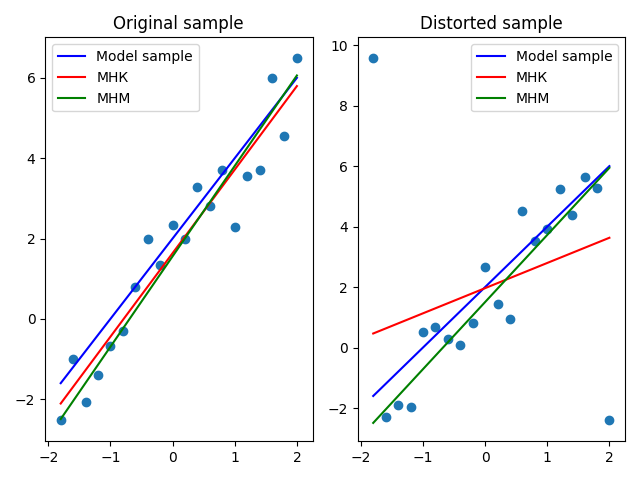
\includegraphics[scale = 0.6]{plt.png} 
    \label{fig:reg}
\end{figure}

\begin{table}[H]
\caption{Таблица оценок коэффициентов линейной регрессии без возмущёний}
\label{tab:my_label1}
\begin{center}
\vspace{5mm}
\begin{tabular}{|c|c|c|}
\hline
& $\overset{\wedge}{a}$ & $\overset{\wedge}{b}$\\
\hline
МНК &2.000&2.000\\
\hline
МНМ &2.08&1.64\\
\hline
\end{tabular}
\end{center}
\end{table}


\begin{table}[H]
\caption{Таблица оценок коэффициентов линейной регрессии с возмущёниями}
\label{tab:my_label2}
\begin{center}
\vspace{5mm}
\begin{tabular}{|c|c|c|}
\hline
& $\overset{\wedge}{a}$ & $\overset{\wedge}{b}$\\
\hline
МНК &2.000&2.000\\
\hline
МНМ &0.83 &1.97\\
\hline
\end{tabular}
\end{center}
\end{table}




\section{Выводы}
По графику \ref{fig:reg} видно, что оба метода дают хорошую оценку коэффициентов линейной регрессии, если нет выбросов. Однако выбросы сильно влияют на оценки по МНК.

Выбросы мало влияют на оценку по МНМ, но ценой за это является б\'oльшая по сравнению с МНК сложность вычисления.



\begin{thebibliography}{}
    \bibitem{numpy}  Модуль numpy  -  https://physics.susu.ru/vorontsov/language/numpy.html
    
    \bibitem{plotlib} 
    Модуль matplotlib - https://matplotlib.org/users/index.html
    
    \bibitem{skp}
    Модуль scipy - https://docs.scipy.org/doc/scipy/reference/
    
\bibitem{lin_reg}
    https://en.wikipedia.org/wiki/Linear\_regression

\bibitem{MNK}
http://www.cleverstudents.ru/articles/mnk.html

\bibitem{6_3}
Шевляков Г. Л. Лекции по математической статистике, 2019.

\bibitem{6_4}
Вероятностные разделы математики. Учебник для бакалавров технических направлений. //Под ред. Максимова Ю.Д. - СПб.:"Иван Федоров 2001. - 592 с.


\end{thebibliography}

\section{Приложения}

Исходники: \url{https://github.com/LanskovNV/math_statistics/tree/master/lab_6}

\end{document}

